Was ist eigentlich so ein Bachelor? Denn mein Englisch-Deutsch-W\"orterbuch
sagt, dass ich mich in einen Studiengang eingetragen habe, in dem ich zum
''Junggesellen der Rechner-Wissenschaft'' gemacht werden soll. Und der
Junggesellenstatus in der Wissenschaft kann nicht wirklich mein Ziel sein, oder?

Wie immer: Don't Panic! Bachelor ist nur ein Name, den die Politik \"ubernommen
hat, um internationaler zu klingen.  So ist das halt bei Hochschulreformen. Und
au{\ss}erdem ist was der Bachelor genau ist erst wichtig wenn ihr fertig seit.
Jetzt ist erstmal wichtig, dass ihr sinnvoll studieren k\"onnt. Und dazu solltet
ihr ein paar Grundlagen wissen.

\textbf{Merke: Das Bachelorstudium ist im Prinzip ein verkorkstes Rollenspiel}

Als erstes gibt es f\"ur Rollenspielfanatiker und Munchkins das offizielle
Regelwerk zum Studium: Die \textsc{\textit{Bachelorordnung}}. Die besteht wie jedes
Regelwerk aus einem kleinen Teil mit Regeln
%TODO:*U NO SAY*
und dem Teil mit den riesigen
Tabellen, die Zeuch beschreiben. Aber anstatt coole R\"ustung und so gibt es
nur Skills. Nur hei{\ss}en die hier Module und man bekommt die erst, wenn man sie
verdient hat.

Au{\ss}erdem gibt es sowas wie XP. Die hei{\ss}en hier aber CP, weil das alles
bitterer Ernst ist und sich deshalb nicht an g\"angige Rollenspiel
Designkonventionen gehalten wird. Und von denen bekommt man etwa einen pro 30
Stunden Studium.

Aber auch das funktioniert irgendwie anders als man das gewohnt ist. Statt dass
man XP bekommt, mit denen man sich bessere Skills holt um dann in Proben
bessere Chancen zu haben, muss man hier erst die Pr\"ufungen bestehen, bekommt
dann das Modul und damit die CP.
%TODO: *DAFU?*.

{\large
\begin{verbatim}
[XP] -> [skills] -> [pruefungen]
[CP] <- [module] <- [pruefungen]
\end{verbatim}}

\textbf{Bacheloraufbau:}
Schauen wir uns also das System mal genauer an.
Das Ziel ist es, den Abschluss Bachelor zu bekommen. Dazu muss man 180CP
bekommen haben, die man mit dem Abschluss von Modulen bekommen hat. Und wie
jeder weiss, muss ein guter Munchkin Min-Maxen. Aber auch das kann der Bachelor
nicht gut.

Um Module abzuschlie{\ss}en, muss man eine Klausur schreiben, eine m\"undliche
Pr\"ufung machen, einen Vortrag halten, gen\"ugend Abgaben gemacht haben, oder
sonst irgendwie gezeigt haben, dass man die CP auch wirklich verdient hat.


\textbf{Die Modulkategorien:}
Die Module sind wie f\"ur Skills, \"ublich in verschiedene Kategorien
eingeteilt. Das kann euch sowohl einschr\"anken als auch Freiheiten geben.
Als erstes sind f\"ur euch die \emph{Basismodule} interessant, denn die m\"usst ihr als Informatiker alle machen.\\
Dann kommen die \emph{Vertiefungsmodule} ins Spiel. Hier kann man seinen Studenten in mindestens drei von f\"unf Kategorien spezialisieren.\\
Die \emph{Anwendungsfachmodule} sind Multiklassenskills, in denen ihr Fertigkeiten aus anderen F\"achern lernen sollt.\\
\emph{Erg\"anzungsmodule} sind durch die \texttt{Gute Idee\texttrademark} entstanden, dass Informatiker mindestens 150 Stunden Soft Skills oder soziales Zeuch gemacht haben sollten. Wir wollen doch keine verschrobenen antisozialen Studenten bauen.\\
Und zum Abschluss gibt es das \emph{Abschlussmodul}, das die Bachelorarbeit und das Oberseminar \"uber die Arbeiten enth\"alt.\\

\begin{center}
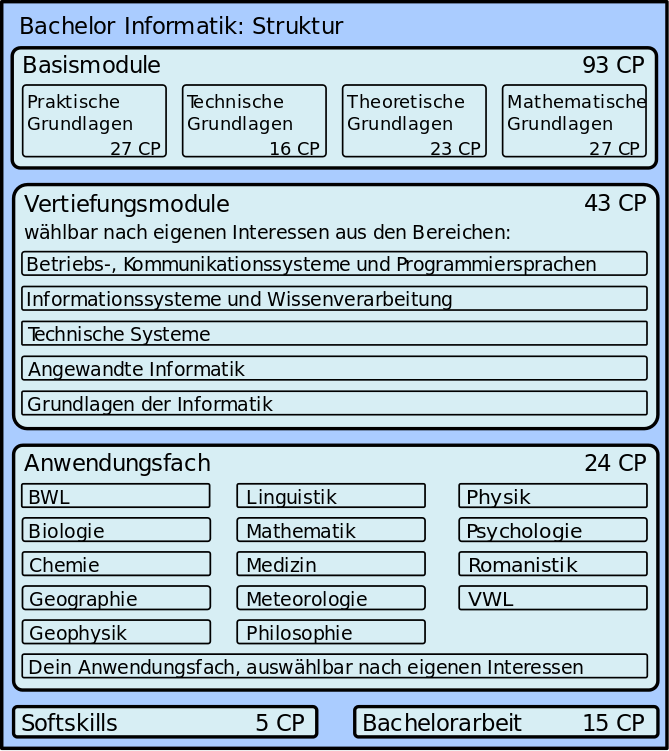
\includegraphics[width=85mm]{bilder/BacInfStruktur}
\end{center}


\textbf{Basismodule:}
Es gibt ein paar Skills die jeder Informatiker haben sollte. Und es gibt
Basismodule. In den Basismodulen lernt ihr offiziell vier Dinge: Mathe, Wie
Computer funktionieren (wird gerne auch ''Hardware'' genannt), Wie man Computer
programmiert und Theoretische Informatik. Das sind alles Vorlesungen, bis auf
das Programmier-Praktikum und das Hardware-Praktikum, die Praktika sind.
Insgesamt gibt es hier 93CP zu holen.

\textbf{Vertiefungsmodule:}
Die gibt es in f\"unf Spezialisierungen: BKSPP, ISWV, TS, ANI und GDI. \emph{''Betriebs-
und Kommunikationssysteme und Progammiersprachen und -paradigmen''} enth\"alt
genau was im Titel steht. \emph{''Informationssysteme und Wissensverarbeitung''}
besch\"aftigt sich mit Textverarbeitung , Datenbanken und k\"unstlicher
Intelligenz. In \emph{''Technische Systeme''} lernt man mehr \"uber Microcontroller,
Rechnerarchitektur und Chipdesign. \emph{''Angewandte Informatik''} ist alles was
sonst nicht untergebracht werden konnte. Da sind dann so Sachen wie
Computergrafik, Zeug und Krempel drin. Wer aber statt Zeug und Krempel lieber
was abgehobenes macht kann in \emph{''Grundlagen der Informatik''} fast schon ein
Mathestudium simulieren. Dort ist mehr Logik, mehr Algorithmentheorie und mehr
Beweise.

Und jetzt kommt der Haken: Du musst mindestens 43CP machen und davon in einem
mindestens 16CP und in zwei anderen mindestens 8CP und die anderen 11CP kannst
du machen wie du willst. Dabei musst du die drei Vertiefungsgebiete, in denen
du leveln willst, dem Pr\"ufungsamt vor der ersten Klausur mitteilen. Alles
klar? OK!

\textbf{Anwendungsfachmodule:}
Die Muliklassenskills auch Anwendungsfachmodule genannt erlauben euch was anderes als Informatik zu lernen.
Die meisten dieser Nebenfachmodule sind geregelt. Das hei{\ss}t, das
Basisregelwerk ''Die Bachelorordnung'' hat vorgefertigte L\"osungen, wie ihr das
Nebenfach machen k\"onnt. Ist euer Nebenfach nicht drin, k\"onnt ihr das trotzdem studieren, aber dann halt ungeregelt.
Dazu muss unser Pr\"ufungsamt mit dem ''gegnerischen'' Pr\"ufungsamt ''kl\"aren'' wie das ganze abgewickelt werden soll.
Fakt ist aber, ihr braucht immer mindestens 24CP.

\textbf{Erg\"anzungsmodule:}
Irgendein schlauer Informatiker hat sich mal gedacht: \emph{Wir wollen, das
Frankfurter Informatiker nicht nur Fachidioten sind, sondern auch ''sozial''
sein k\"onnen. Die haben dann ''Soft Skills''. Wie ''Teamf\"ahigkeit'' und so. Und das
ist dann gut.} Aber da zu viel Soziales nicht in den Studienverlausplan passt, macht ihr 5CP.
Da ist dann auch die Studienorientierung STO drin. Die im ersten Semester 2CP gibt, und sp\"ater nur noch halb so viel.
Da wird euch nochmal wie man studiert auf dem Silbertablett gereicht.

\textbf{Die restlichen 15CP:}
Gibt es mit der Bachlorarbeit.

\textbf{Die Bachelorarbeit:}
Das ist sowas wie eine echte wissenschaftliche Arbeit. Wenn ihr die gamcht habt, gibt das 15CP im Abschlussmodul.

\begin{center}

\includegraphics[width=\linewidth]{comics/exercise}\\
\end{center}

\textbf{Die Klausurregeln:}
Und nun steigt die Spannung. Die Klausurphase beginnt.
W\"ahrend im Semester Wochen vergehen k\"onnen, ohne dass viel passiert, ist die Klausurphase eher wie Kampfrunden.
Eine Megasekunde, die im echten Leben vergeht, kommt einem wie eine Gigasekunde an der Uni vor.
    Aber keine Panik, es gibt einige Tricks und ein paar Regeln, die ihr
anwenden k\"onnt, um sinnvoll lebendig, und mit ein paar mehr CP durch die
Klausurphase zu kommen.

\textbf{Anmeldung:}
Zu Klausuren m\"usst ihr euch zwei Wochen vorher angemeldet haben. Und vor der ersten Klausur m\"usst ihr euch f\"ur den Bachlor anmelden.
Wenn ihr die Klausur schreibt und nicht angemeldet seit, gibt das keine CP.

\textbf{Timing:}
Zuerst ist wichtig zu planen, wann ihr Klausuren schreibt.
Die Termine selbst k\"onnt ihr zwar nicht \"andern, aber ein guter Munchkin hat die Bachelorordnung gelesen
und hat festgestellt, dass viele Klausuren jedes Semester angeboten werden.

Aber wie soll es mir helfen, die Klausur zu verschieben?
N\"achstes Semsester sind doch wieder Klausuren, oder?

Aber da ist es wichtig
zu wissen, wie die Professoren diese Regel mit jedem Semester auslegen.
Professoren waren alle mal Studenten und sind deshalb fast so faul wie wir.
Und fast immer m\"ussen Nachklausuren angeboten werden, f\"ur Studenten, die durchgefallen sind oder nicht teilnehmen konnten.
W\"ahrend die Vorlesungen meisstens in der dritten April- oder Oktoberwoche, anfangen f\"angt das Semester p\"unklich am Ersten an.

Und deshalb sind die Nachklausuren meistens am Ende der Semesterferien, aber im neuen Semester. Der
ge\"ubte Munchkin braucht also seine Klausuren nicht alle auf einmal zu
schreiben, sondern lernt am Anfang \emph{und} am Ende der Semesterferien.
Ansonsten gilt: \textbf{Konzentrier dich auf wenige Klausuren, statt in allen zu versagen.}
\emph{Bla, bla, lernt rechtzeitig, bla\dots}\\

\textbf{Freiversuche - Rerolls f\"ur Klausuren:}
Und jetzt kommen die kleinen Feinheiten des Regelwerks, die jeden Munchkin interessieren sollten.
Ger\"uchteweise haben manche Studenten Klausuren mitgeschrieben und kl\"aglich versagt. Daran ist noch nichts besonderes.
Aber f\"ur diese Studenten war es so, als h\"atten sie die Klausur nie
geschrieben und haben sich einfach beim n\"achsten mal wieder in die Klausur
gesetzt. Und noch viel besser. Andere, die grad so bestanden hatten, sa{\ss}en
in der Klausur und konnten nochmal mitschreiben und haben am Ende eine bessere
Note gehabt. Wie geht das?

Naja, eigentlich ist nichts besonderes daran. Wenn du innerhalb der
Freiversuchsfrist eine Klausur schreibst, kannst du beim ersten Mal
durchfallen, ohne dass das als Fehlversuch gez\"ahlt wird.
Die Freiversuchsfrist ist in der Bachelorordnung festgelegt und ist an den Studienverlauf angepasst.
Das soll euch dazu motivieren, die Klausur zu beim erstem Mal oder in der Nachklausur mitzuschreiben.
Das funktioniert aber nur in den Basismodulen so. In den Vertiefungs- und Anwendungsfachmodulen funktioniert das leider nicht.
Aber die Basismodule machen \"uber die H\"alfte des Studiums aus, also ist das gar nicht so schlecht.

Und wer wider Erwarten die Klausur besteht und mit seiner Note nicht zufrieden
ist, kann die Klausur nochmal schreiben. Dazu muss man sich nach der Klausur
f\"ur die n\"achste Klausur anmelden. Das kann man aber auch nur in den
Basismodulen und insgesamt nur f\"unf mal. Da es aber nur 9 Klausuren in den Basismodulen gibt,
ist das immer noch viel. Aber die genauen Regeln bekommt ihr noch rechtzeitig in der Studienorientierung erz\"ahlt.

\textbf{Studienorientierung:}
\textbf{
Die Studienorientierung ist soooo wichtig, dass wir einen extra Artikel geschrieben haben. Macht die im ersten Semester und alles wird gut. Ausserdem haben wir diesen Absatz extra fettgedruckt!}

\textbf{FAIL - Das Howto:}
Manchmal muss man einfach alle Br\"ucken hinter sich lassen. Und manchmal will man nicht gehen, sondern rausfliegen. Und so gehts:

\textbf{FAIL - Die Sparsame Methode:}
Bezahl deine Studiengeb\"uhren nicht. So einfach ist das. Die bezahlt man sonst immer im Januar oder im Juli. Aber wer wirklich raus will, findet in der Sparsamkeit eine wirksame Methode.

\textbf{FAIL - Die Faule Methode:}
Mach in den ersten drei Semestern weniger als 15CP. Das sind so ungef\"ahr zwei Module von zehn. Dann musst du nur noch die Anfragen vom Pr\"ufungsamt ignorieren und keine Fristverl\"angerung beantragen. Dann bist du raus.

\textbf{ULTRAFAIL - Die Wahre Methode:}
Wenn du nicht nur rausfliegen willst, sondern gar nicht mehr Informatik
studieren k\"onnen willst, solltest du dreimal durch eine Pr\"ufung in einem
Basismodul durchfallen (viermal, wenn du schon in der Freiversuchsfrist
anf\"angst). Wer eine Pr\"ufung dreimal nicht besteht, hat ''endg\"ultig nicht
bestanden''. Und wenn das soetwas grundlegendes wie Programmierung ist, kannst
du nicht mehr Informatik studieren, auch nicht woanders in Deutschland. Auch
hier musst du darauf achten, alle Beratungsgespr\"ache zur\"uckzuweisen.

\textbf{N\"utzliche Tips:}
\emph{bla, bla, \"Ubungsabgaben, yadda, yadda, Lernen, bla, blubber, Zeiteinteilung, bla, regelm\"a{\ss}ig da sein, trololo, Durchhalteverm\"ogen, bla, generische Motivationsrede\dots}\\

\textbf{Und nun?}
Naja, da sind noch mehr Seiten in der Don't Panic! 42. Die k\"onnt ihr auch
lesen. Wichtig ist vor allem, sich an der Uni einzuleben, wenn man erfolgreich
studieren will. Und das sieht f\"ur jeden anders aus. Manche machen ihr Studium
schnell und andere lassen sich Zeit. Und wichtiger als die Skills, die ihr hier
bekommt, ist die Erfahrung. Wenn ihr hier fertig seit, m\"usst ihr eh wieder
neue Sachen lernen.





